\vspace{-5pt}
\section{A Case Study of Cross-point ReRAM Macro Design}\label{sec:macro}
Since the array size of a cross-point ReRAM array is strictly limited by
reliability requirements, the design of a ReRAM macro is greatly different
from the traditional DRAM design. A cross-point ReRAM macro is implemented
by establishing a large amount of small cross-point arrays with
appropriate peripheral circuity and organizations. In this section, we
evaluate the area, energy consumption, and bandwidth of a 256 Mbits ReRAM
macro. We apply the similar memory organization as Kawahara's
work~\cite{crossbar_Panasonic}. The 256 Mbits ReRAM macro consists of
eight planes, each of which is 32 Mbits. Each plane has separate wordline
decoder, bitline selectors, sense amplifiers, and write circuity. Due to
limitations of space, we only present the results of ReRAM macro
implemented by four different typical cell parameters: ($Kr=20,
I_w=40uA$), ($Kr=20, I_w=200uA$), ($Kr=40, I_w=40uA$), and ($Kr=40,
I_w=200uA$). For each of them, we vary the number of bit per write to
investigate the relation among the area, energy consumption, and bandwidth
of the ReRAM macro.


%Figure~\ref{fig:aaable}
Table~II shows the total area, energy consumption, and bandwidth of the
256 Mbits ReRAM macro. Clearly, consistent to our previous discussion, the
total area and energy consumption of the ReRAM macro increase with the
increase of nonlinearity, the scaling of write current, as well as the
increase of the number of array-level bits per write. Besides, the
bandwidth also has the similar trend as area and energy consumption. This
observation implies that we have to either sacrifice the area efficiency
or increase the energy budget to improve the bandwidth of the ReRAM macro.

We also investigated three other important design metrics: bandwidth per
nanojoule ($BW/nJ$), bandwidth per square millimeter($BW/mm^2$), as well
as bandwidth per nanojoule per square millimeter ($BW/(nJ\cdot mm^2)$).
Bandwidth per nanojoule reflects the energy efficiency on the bandwidth.
The higher the bandwidth and the less amount of energy used to achieve a
larger values of this metric. Besides, since the area is directly related
to the cost, bandwidth per square millimeter is a good indicator of the
economics of the bandwidth. As shown in Figure~\ref{fig:BWpAE} the
bandwidth per nanojoule for single-bit write is always better than that
for multi-bit write operation. Besides, there also exist a optimal number
of bits per write for multi-bit write schemes: 32 bits for the cell with
Kr=20, and 8 bits for cells with Kr=40. However, from the bandwidth per
square millimeter point of view, the cells with different write current
have different situation: for cells with large write current
($I_w=200uA$), optimal number of bits per write is 16 bits. On the other
hand, if the write current scales to $40uA$, the bandwidth per square
millimeter increases monotonically with the increase of write bit number,
and the large number of bit per write is favorable. The reason for this
different is that, for the cell with large write current, the wordline
drivers and bitline multiplexors can no longer be hidden underneath the
array, which impact the area efficiency of the entire macro.
Figure~\ref{fig:BWpAE2} shows the bandwidth per nanojoule per square
millimeter results. Similarly, this metric also has a optimal number of
bits per write for different cells: 8 bits for the cell with Kr=20, and 4
bits for cells with Kr=40. However, we should note that, even for the same
ReRAM cell, the ``sweet spot'' for different metric is different.
Therefore, we can conclude that the optimal configuration varies with the
optimization target($BW/nJ$, $BW/mm^2$, or $BW/(nJ\cdot mm^2)$).

%\begin{figure}[!t]
%\centering\label{fig:aaable}
%  % Requires \usepackage{graphicx}
%  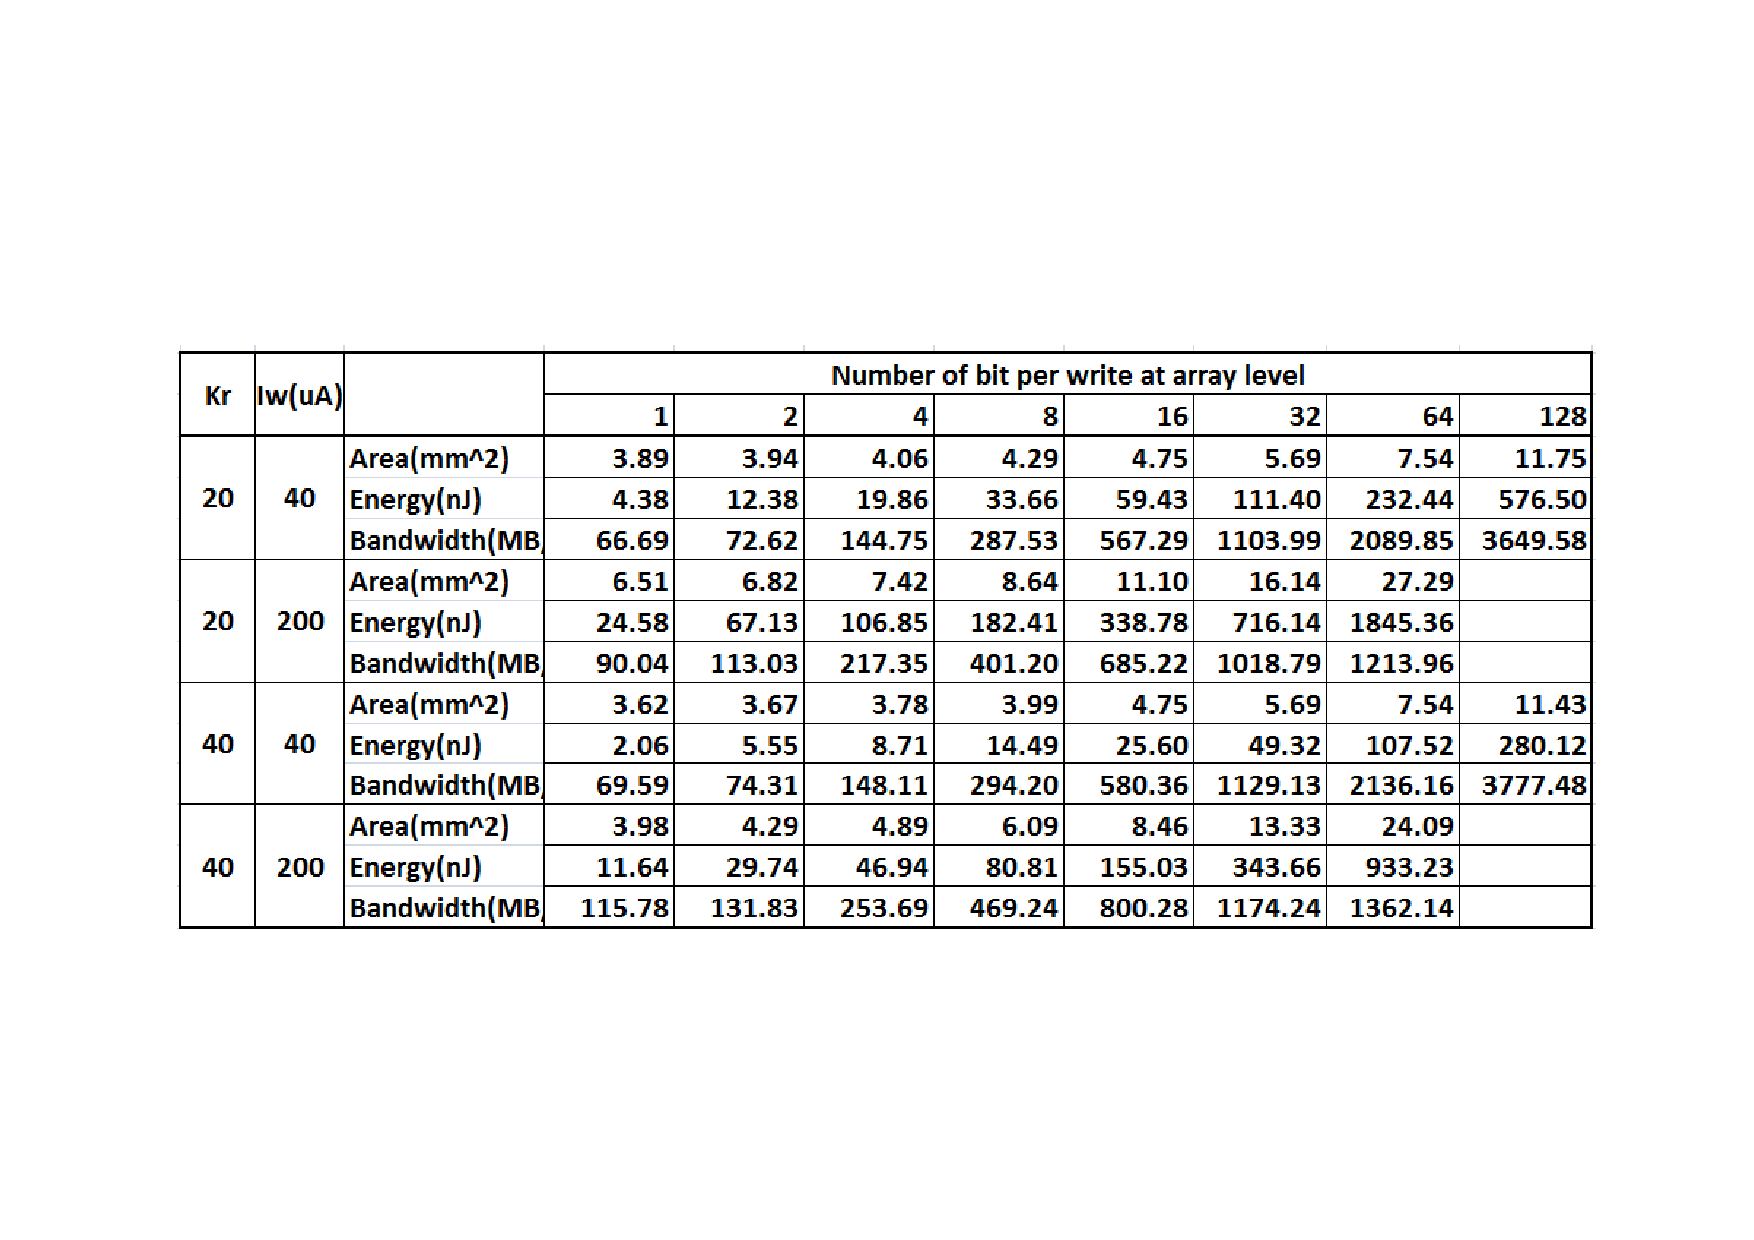
\includegraphics[width=0.5\textwidth]{./figures/Table}\\
%  \caption{Area, energy, and bandwidth results of 256 Mbits ReRAM macro.}
%  \vspace{-5pt}
%\end{figure}


%\begin{figure}[!]
%\centering\label{fig:EpJ}
%  % Requires \usepackage{graphicx}
%  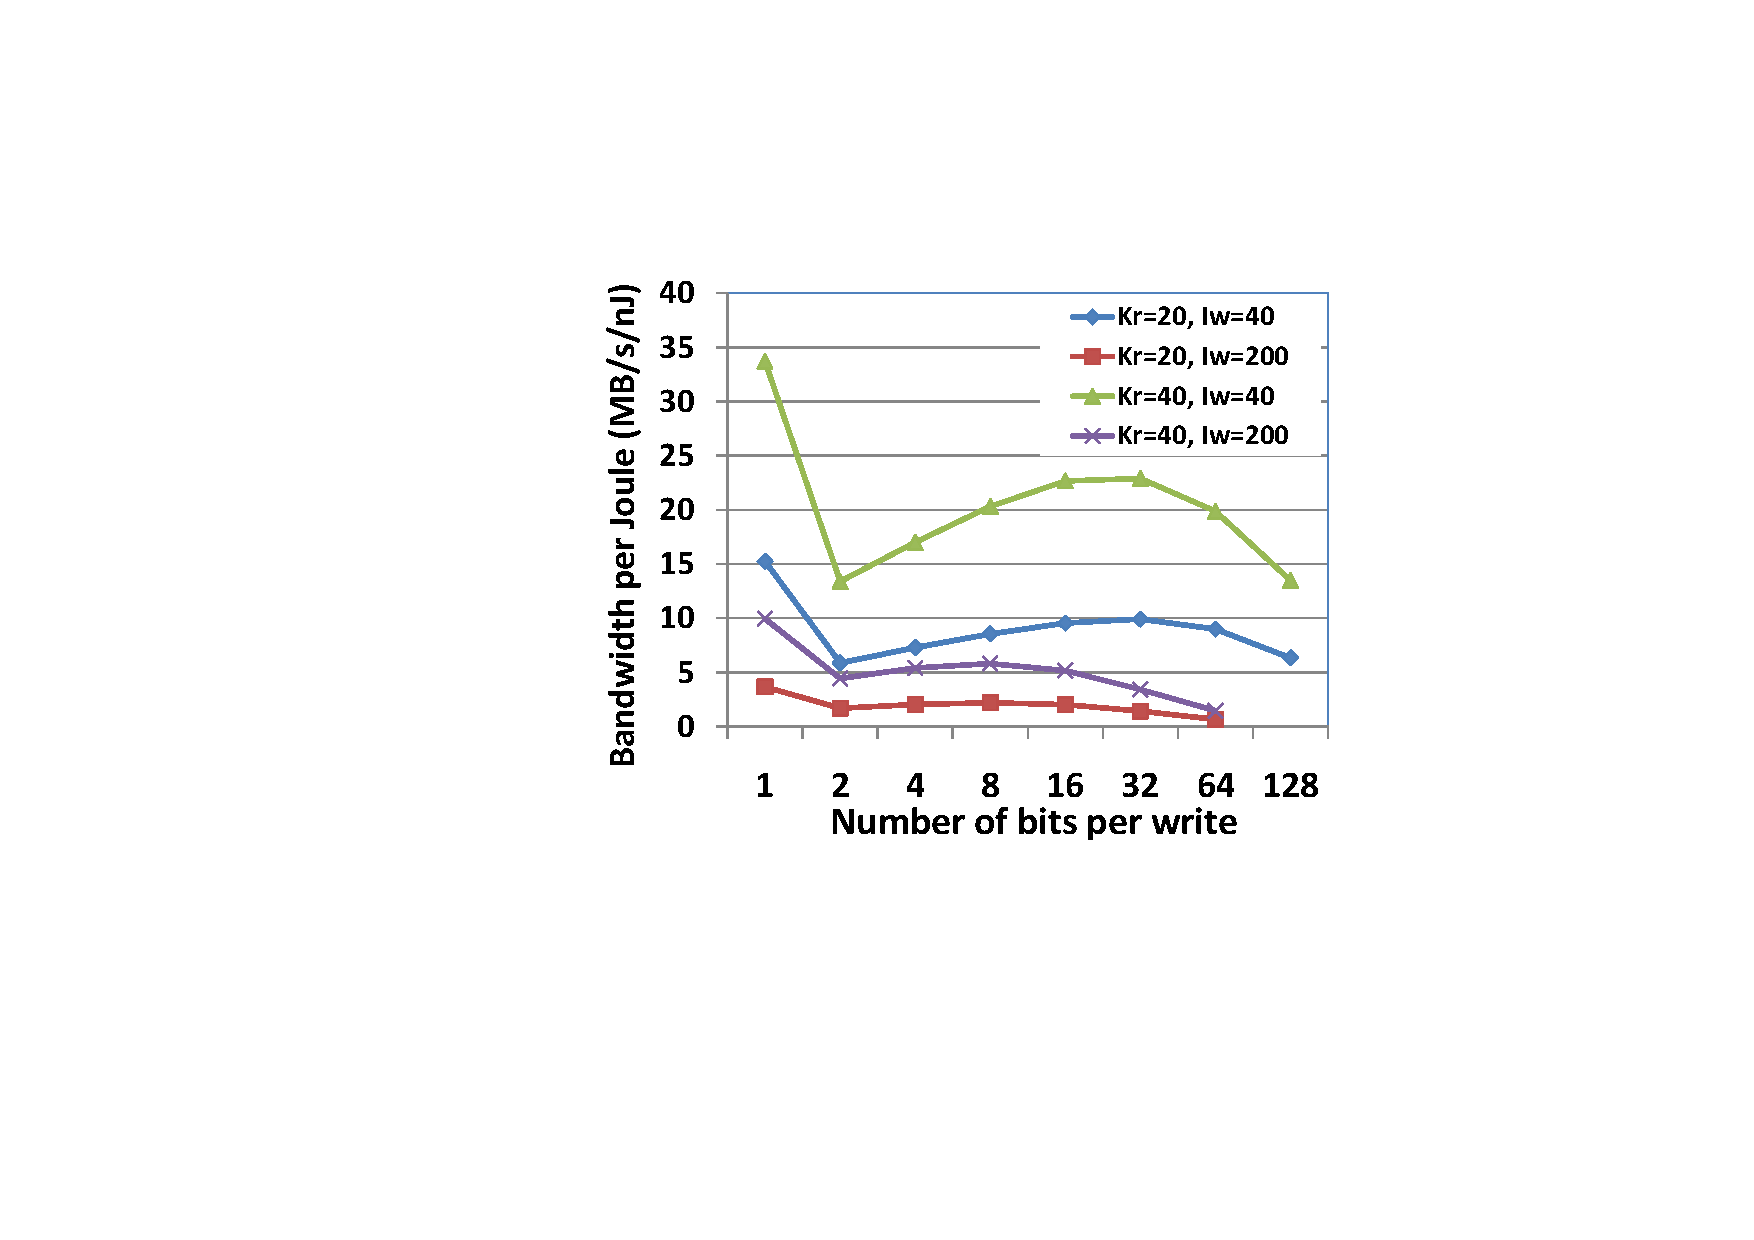
\includegraphics[width=2.3 in]{./figures/EpJ2}\\
%  \caption{Bandwidth-per-Joule of 256 Mbits ReRAM macro.}
%  \vspace{-15pt}
%\end{figure}


\begin{figure}[!]
\centering\label{fig:BWpAE}
  % Requires \usepackage{graphicx}
  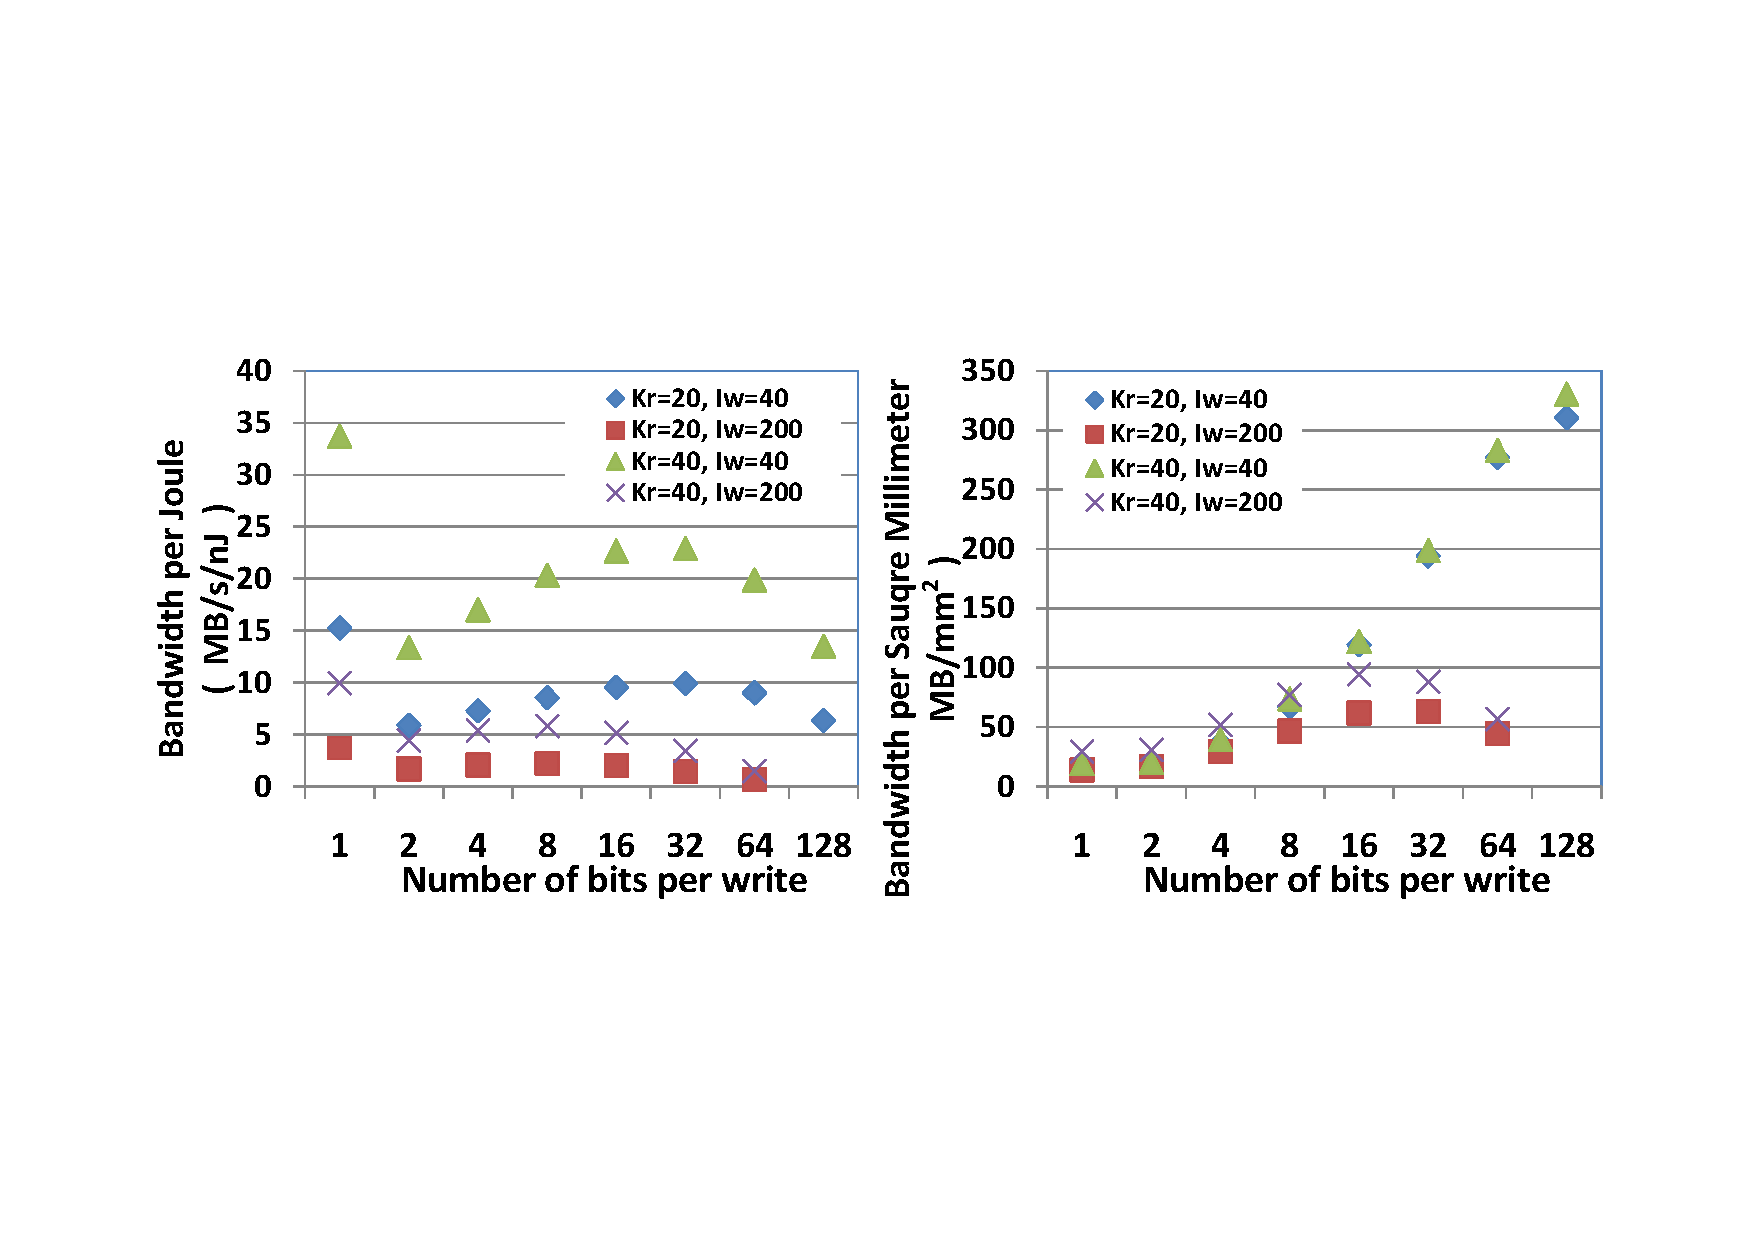
\includegraphics[width=3.4 in]{./figures/BWpAE}\\
  \caption{Bandwidth-per-Joule of 256 Mbits ReRAM macro.}
  \vspace{-5pt}
\end{figure}
\begin{figure}[!]
\centering\label{fig:BWpAE2}
  % Requires \usepackage{graphicx}
  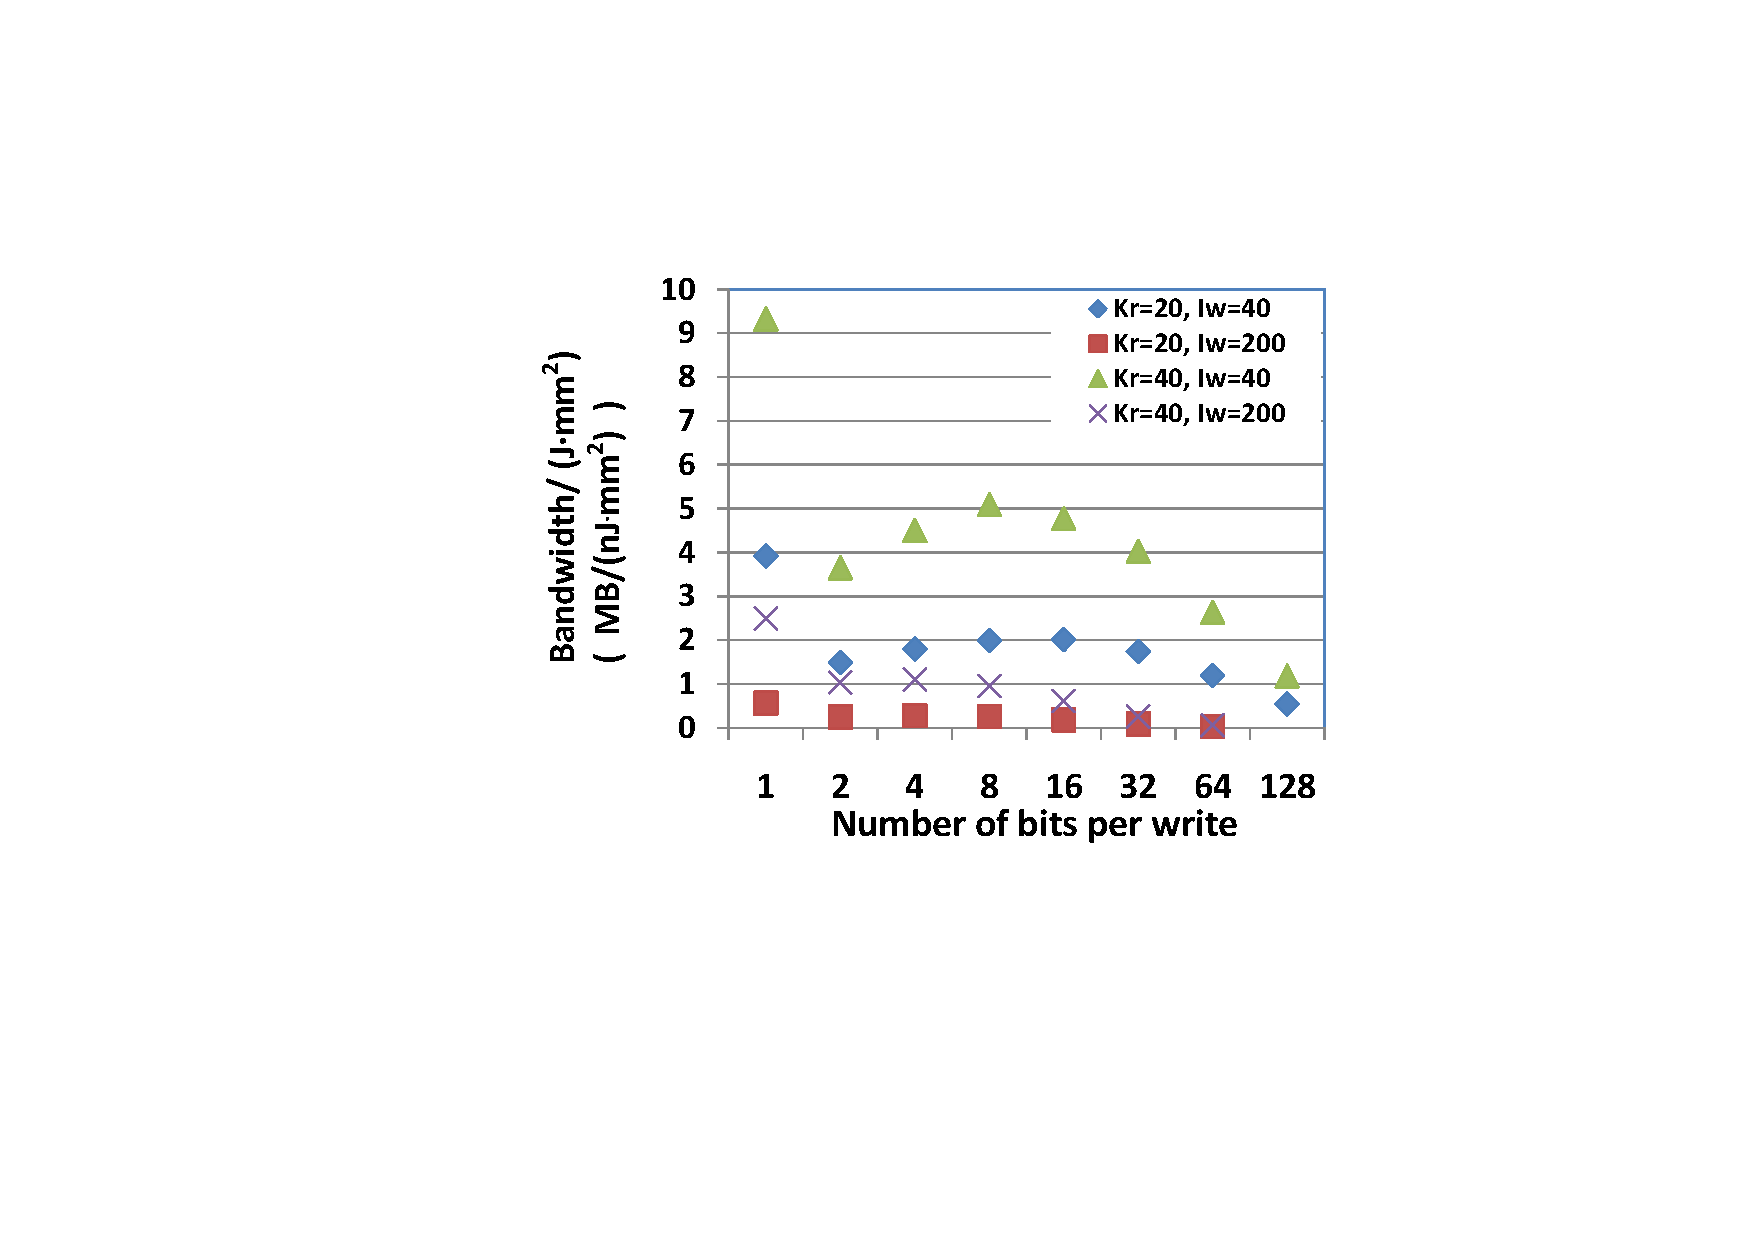
\includegraphics[width=2 in]{./figures/BWpAE2}\\
  \caption{Bandwidth-per-Joule of 256 Mbits ReRAM macro.}
  \vspace{-15pt}
\end{figure}
